\documentclass{beamer}
\usepackage[utf8]{inputenc}
\usepackage[T2A]{fontenc}
\usepackage[serbian]{babel}
\usepackage{graphicx}
\usepackage{caption}


\title{Klasifikacija filmskih žanrova u odnosu na muziku iz filma}
\author{Dunja Mijačić 74/2019}
\date{\today}

\begin{document}

\frame{\titlepage} 

\begin{frame}{Filmski Žanrovi}
\begin{itemize}
\item \textbf{Romantika:} Muzika za romantične filmove često se karakteriše nežnim melodijama i složenim harmonijama. Ova vrsta muzike prenosi ljubav, strast i romantični doživljaj. Žičani instrumenti često dominiraju u ovakvim kompozicijama.

\item \textbf{Mjuzikl:} Mjuzikli su poznati po svojim veselim i melodičnim pesmama. Muzika za mjuzikle često integriše pesme i ples u priču filma. Ova vrsta muzike podstiče energiju i emocionalnu izražajnost.

\item \textbf{Vestern:} Za vestern filmove, muzika je često inspirisana zapadnim temama i tradicijama. Upotreba gitare, harmonike i glasova najavljuje ovaj žanr. Muzika je obično melanholična i prikazuje teške uslove i borbu na divljem zapadu.

\end{itemize}
\end{frame}

\begin{frame}{Filmski Žanrovi}
\begin{itemize}
\item \textbf{Horor:} Muzika u horor filmovima ima za cilj da izazove napetost i strah kod gledalaca. Tamni i jednostavni zvuci, uz upotrebu orgulja i udaraljki, stvaraju uzbudljivu i neizvesnu atmosferu. Muzika često ima neobične i distorzirane zvukove.

\item \textbf{Naučna fantastika (Sci-Fi):} Muzika za naučno-fantastične filmove često je futuristička i elektronska. Sintisajzeri i kompjuterski generisani zvukovi doprinose prikazu budućnosti i neizvesnosti. Melodije su obično kompleksne i ambijentalne.
\end{itemize}
\end{frame}

\begin{frame}{Slike Filmskih Žanrova}
\centering
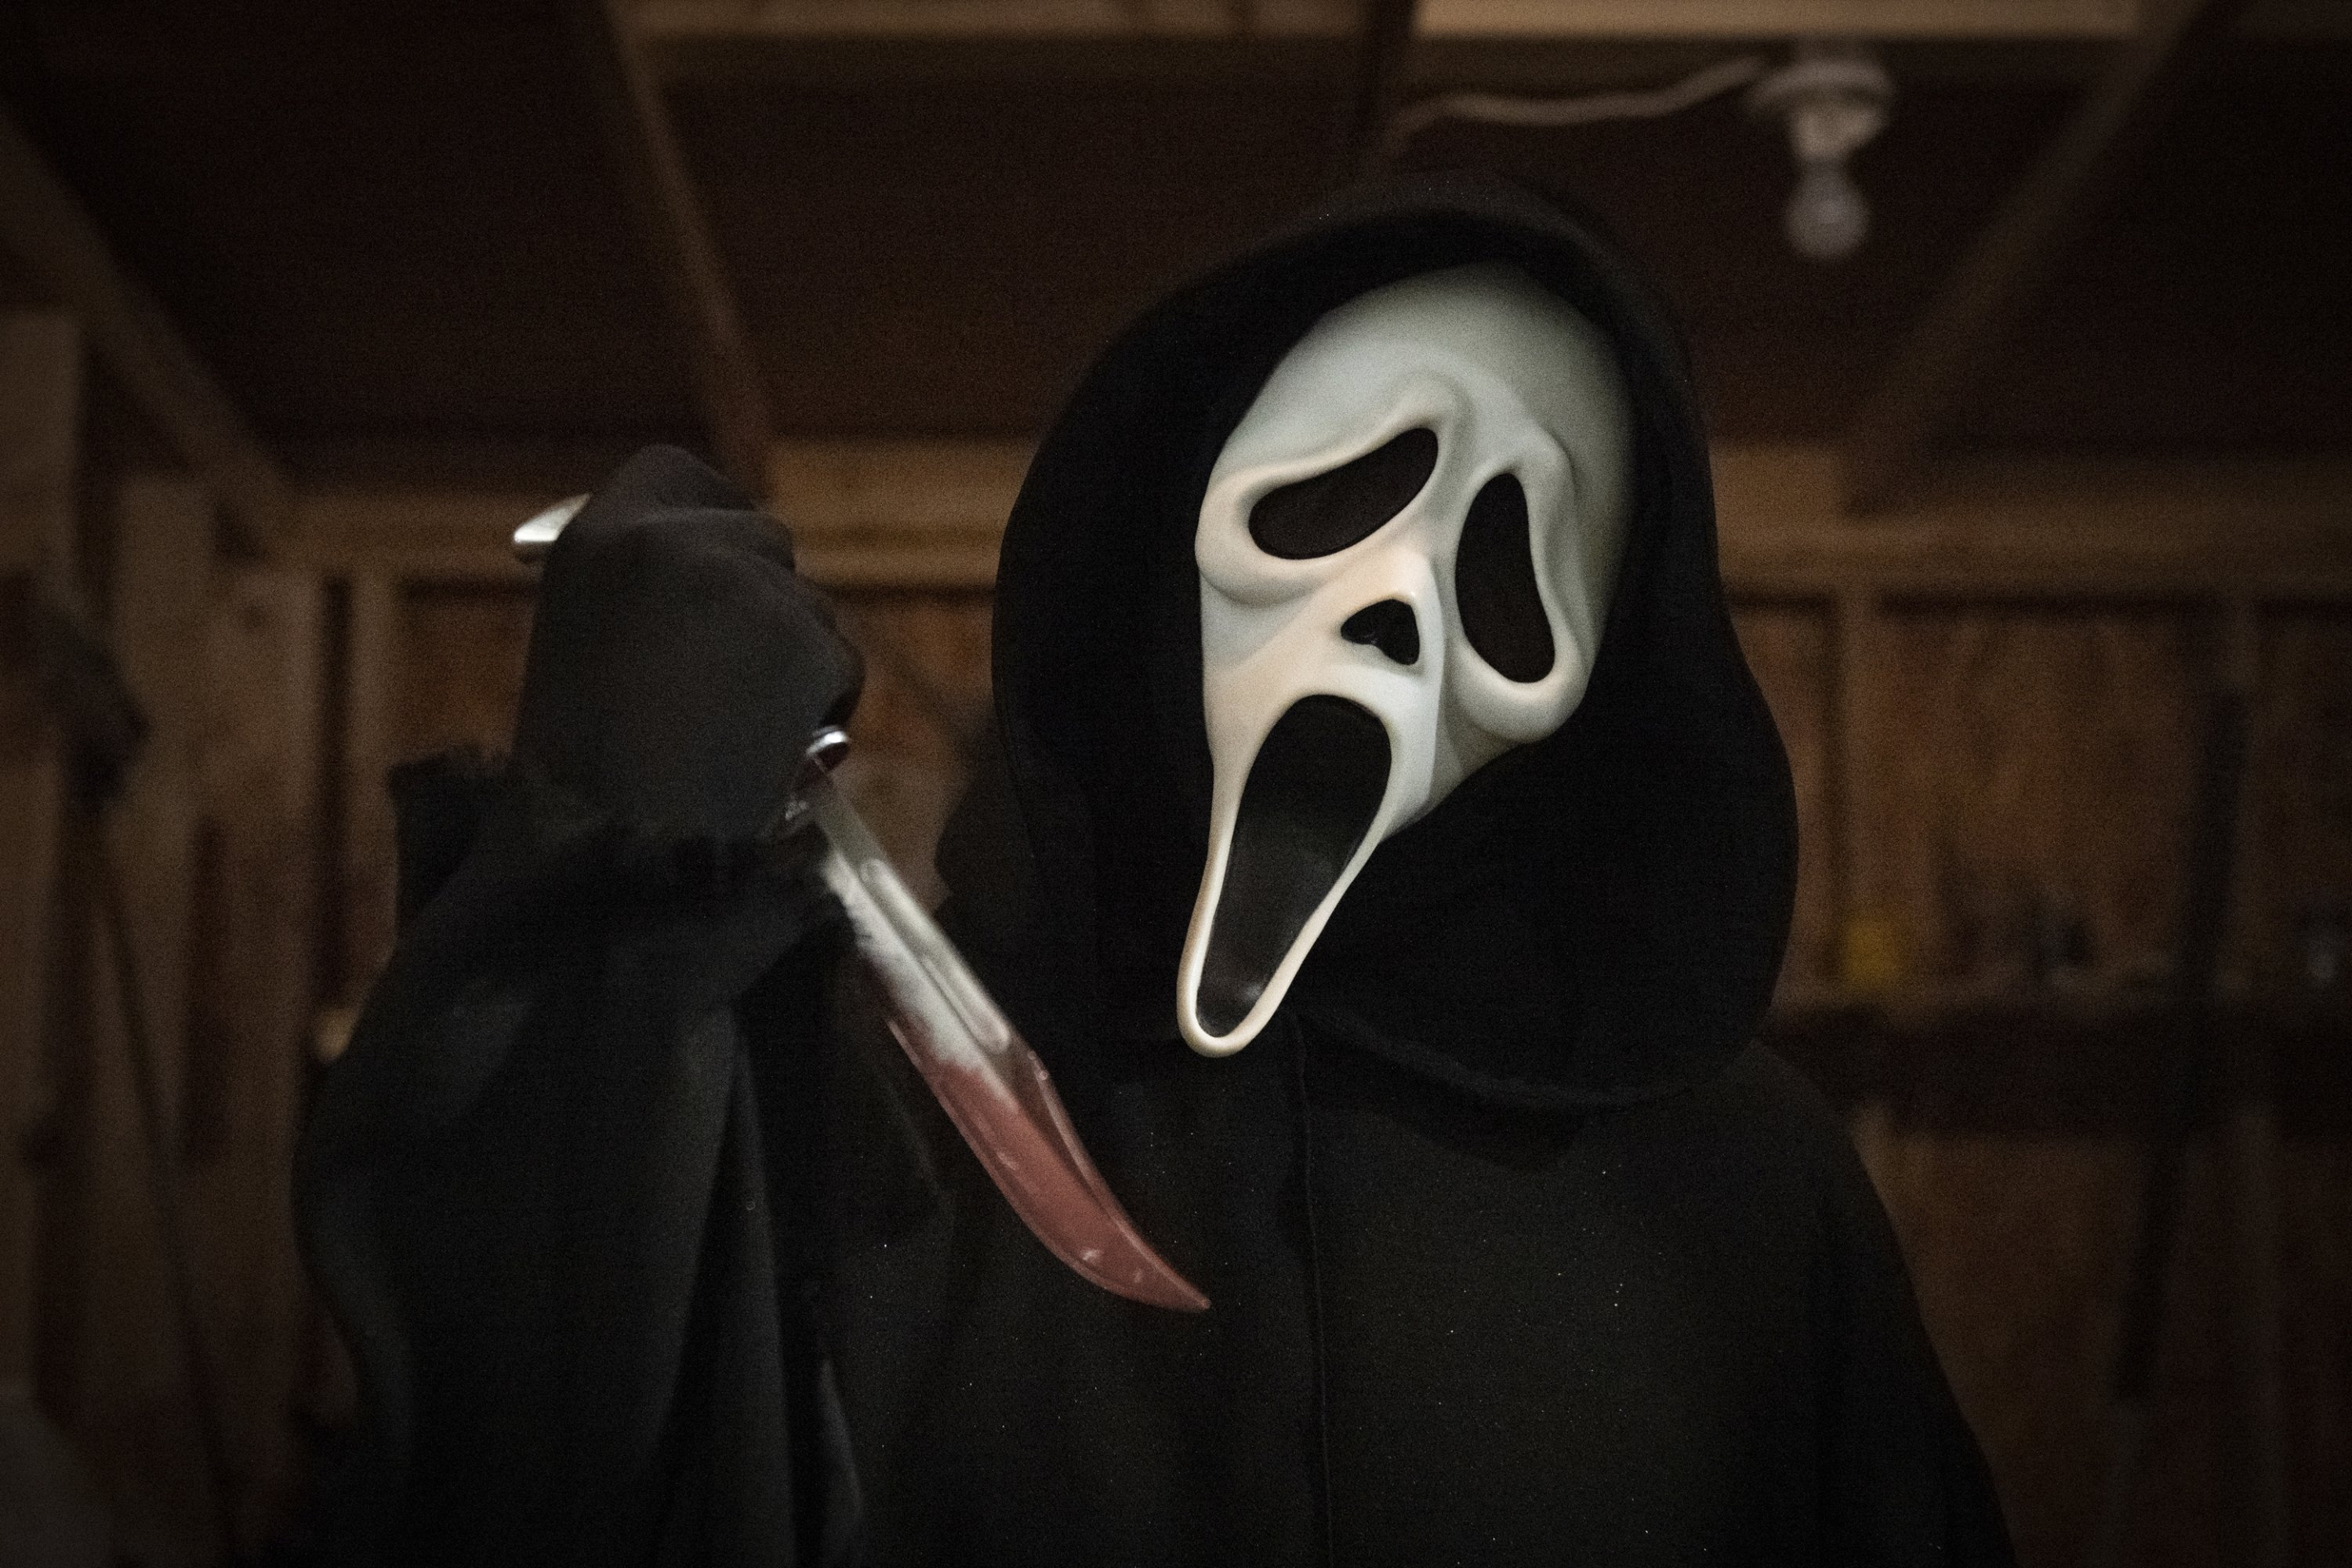
\includegraphics[width=0.4\linewidth]{slike/horor.jpg}
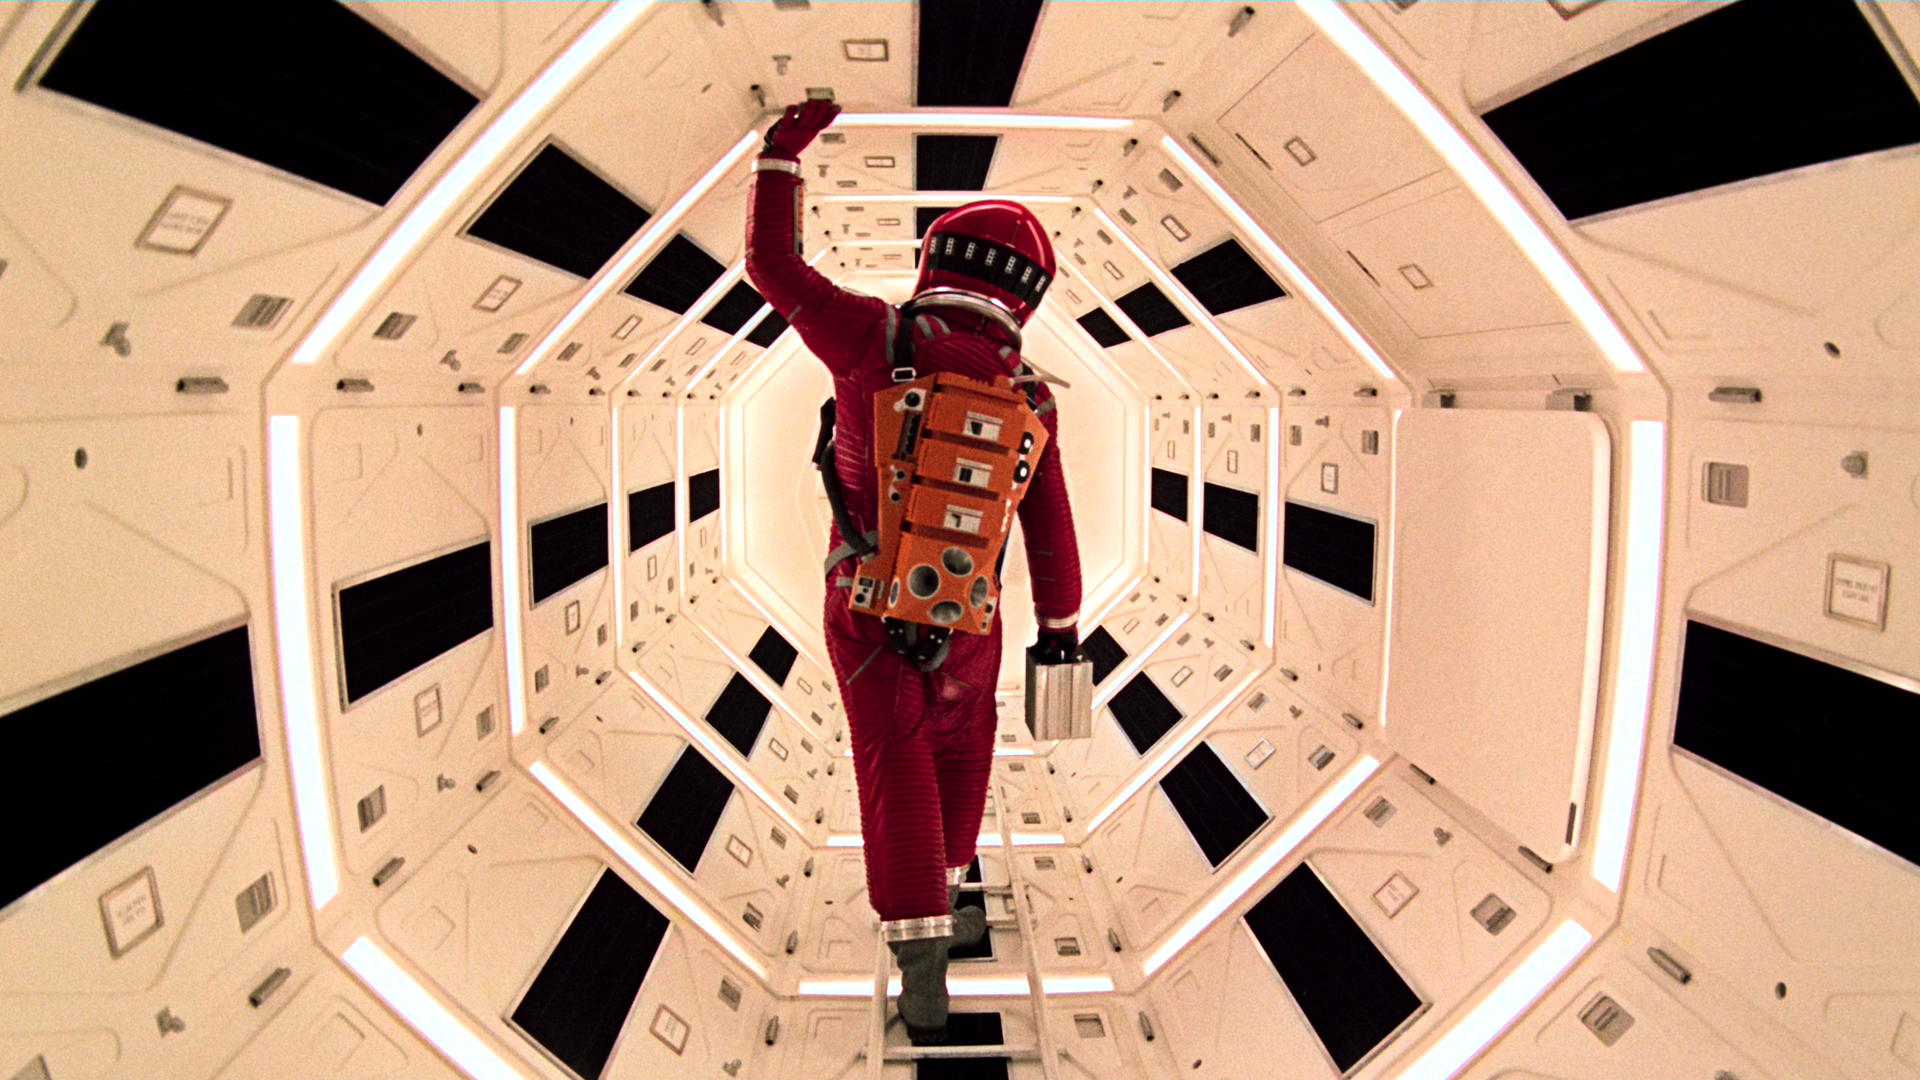
\includegraphics[width=0.4\linewidth]{slike/odiseja.png}\\
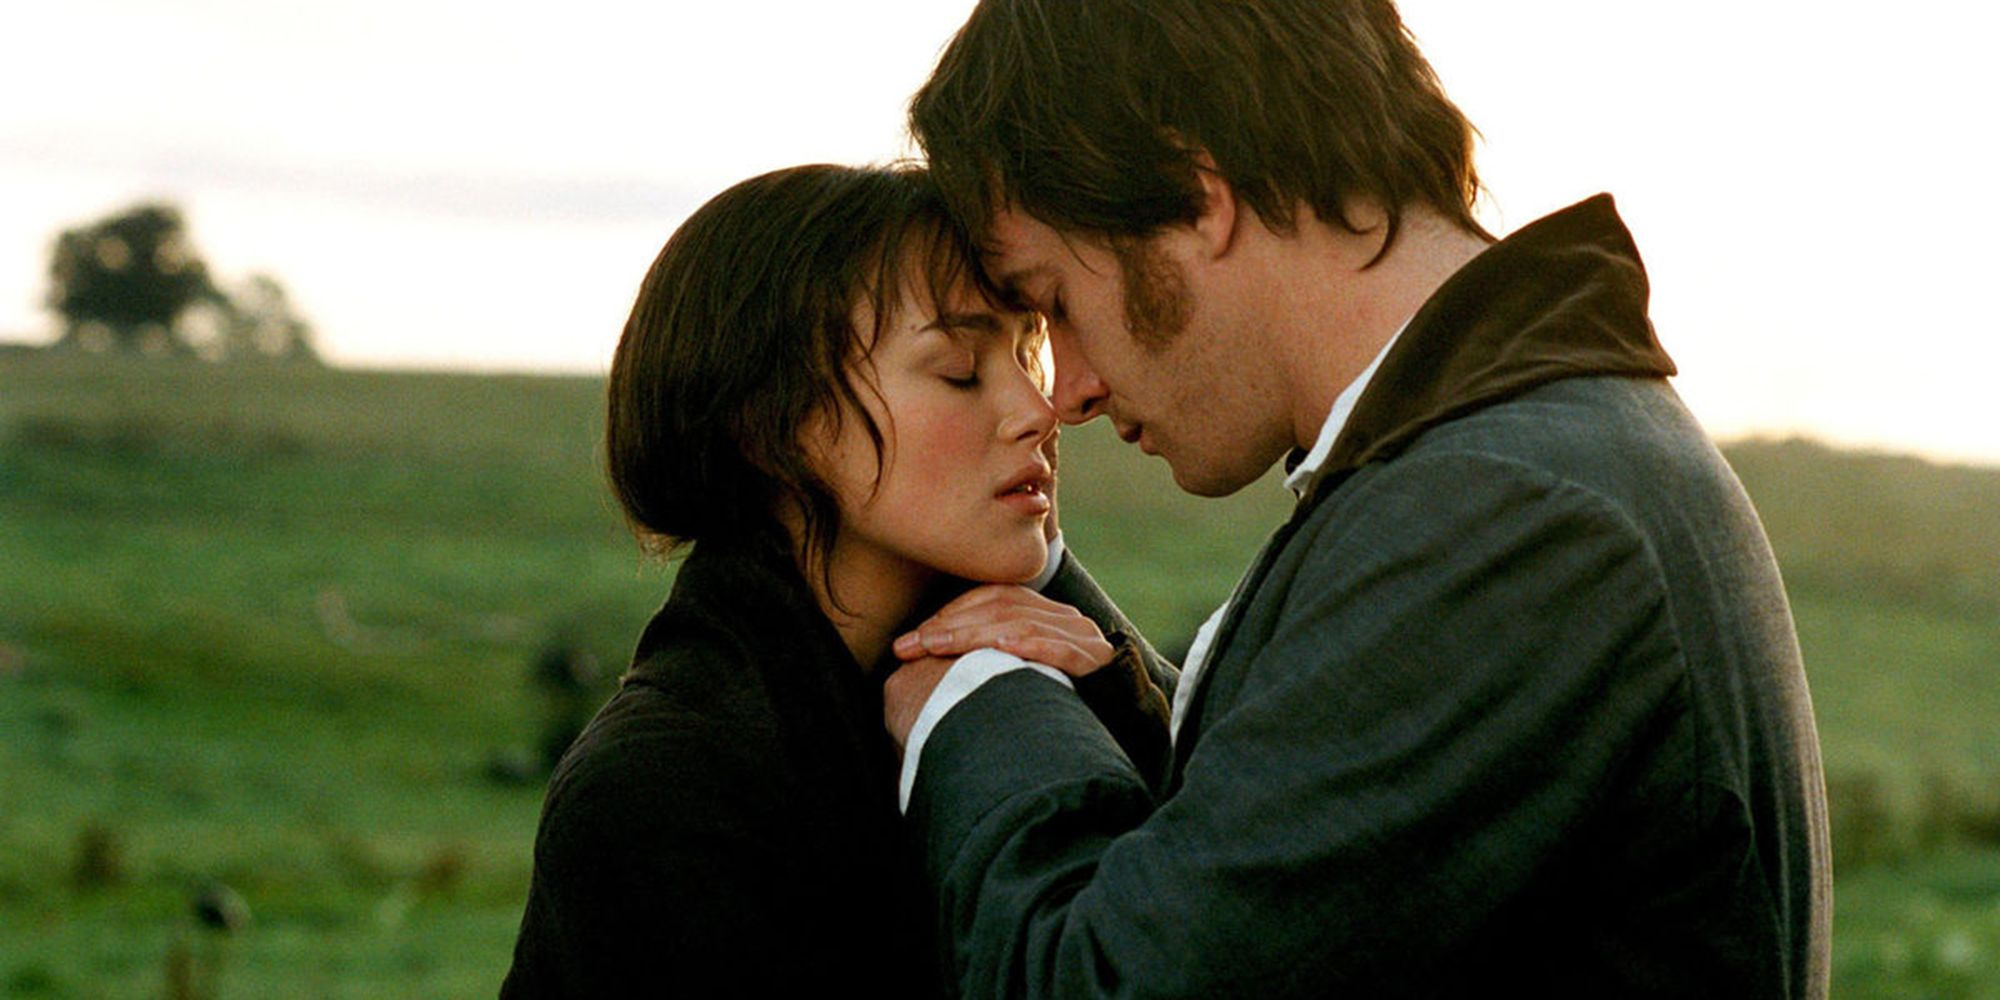
\includegraphics[width=0.3\linewidth]{slike/romantic.jpg}
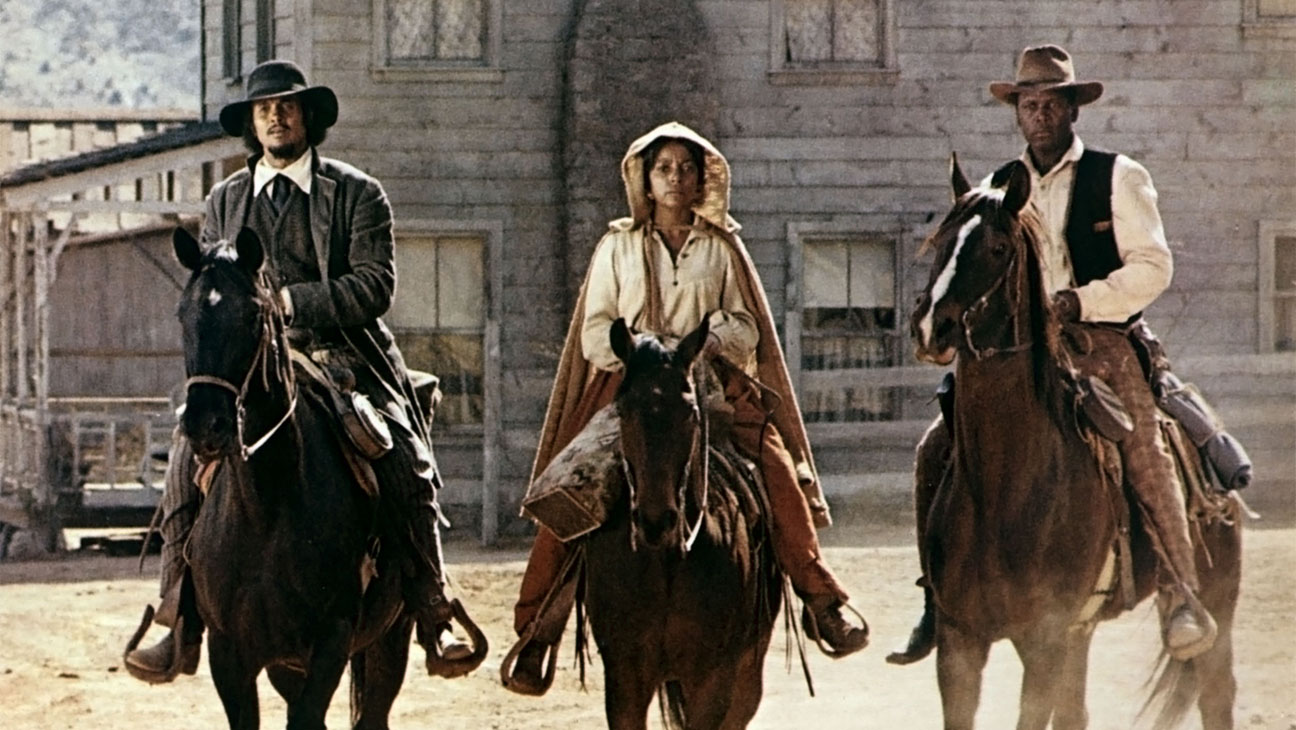
\includegraphics[width=0.3\linewidth]{slike/western.jpg}
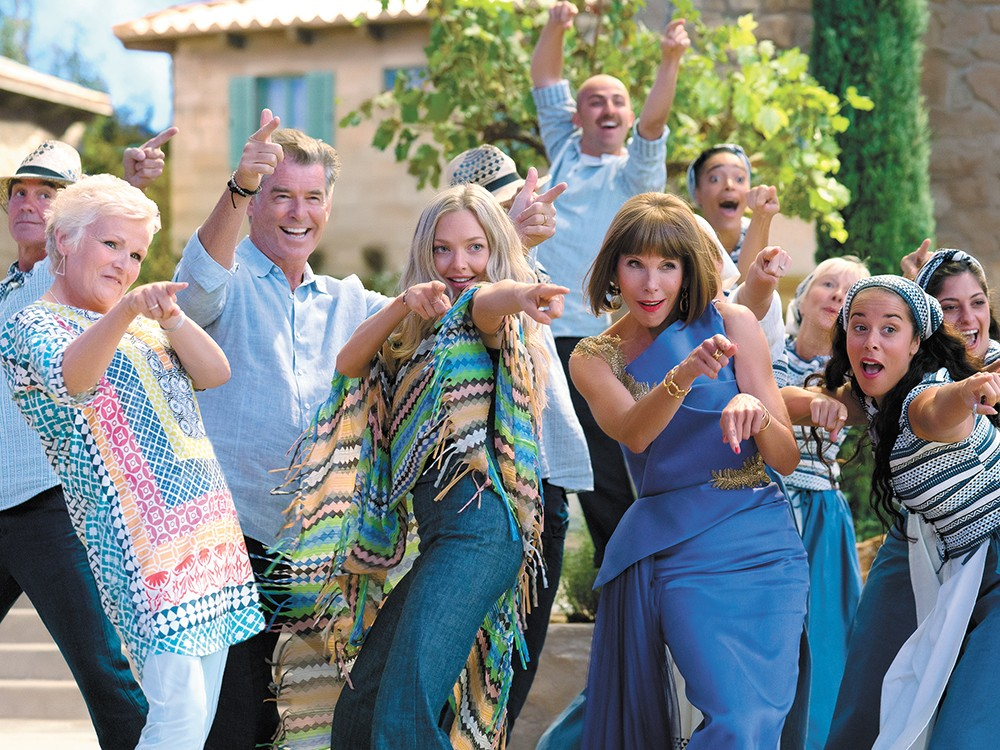
\includegraphics[width=0.3\linewidth]{slike/musical.jpg}
\end{frame}



\begin{frame}{Librosa Biblioteka}
\centering
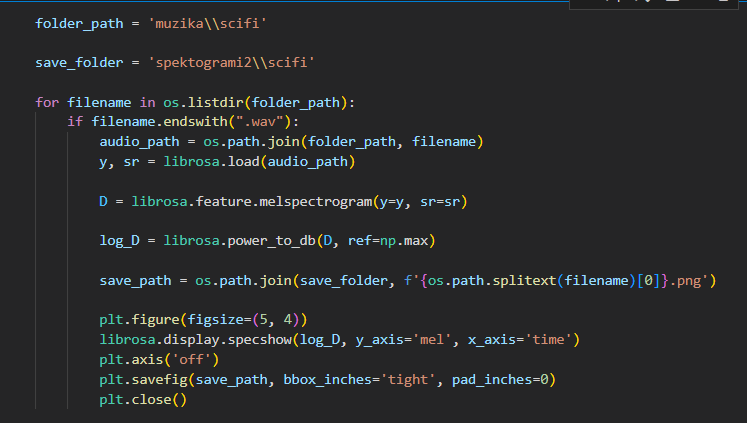
\includegraphics[width=0.9\linewidth]{slike/librosa.png}
\end{frame}

\begin{frame}{Spektrogrami}
Vizuelna reprezentacija audio signala koja prikazuje frekvencijski domen signala u zavisnosti od vremena. Koristi se za analizu i obradu audio podataka.

\end{frame}

\begin{frame}{Spektrogrami Žanrova}
\centering

\begin{minipage}{0.3\linewidth}
  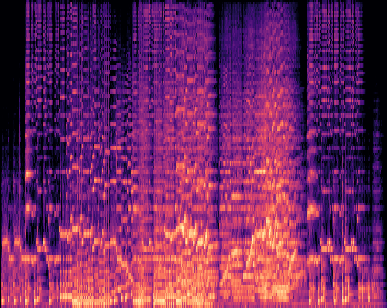
\includegraphics[width=\linewidth]{slike/western06.png}
	Western
\end{minipage}%
\begin{minipage}{0.3\linewidth}
  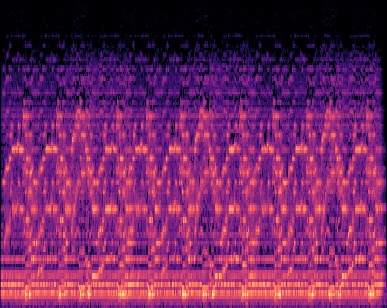
\includegraphics[width=\linewidth]{slike/scifi48.png}
	Sci-fi
\end{minipage}%
\begin{minipage}{0.3\linewidth}
  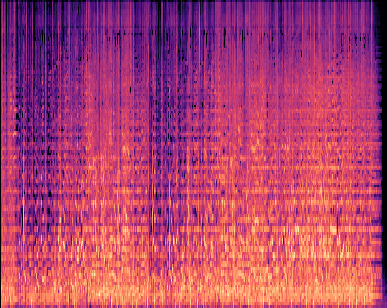
\includegraphics[width=\linewidth]{slike/romantic00.png} 
	Romantic
\end{minipage}%
\end{frame}

\begin{frame}{Spektrogrami Žanrova}
\centering

\begin{minipage}{0.4\linewidth}
  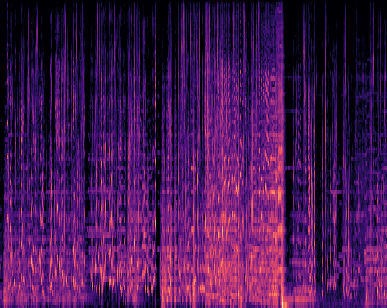
\includegraphics[width=\linewidth]{slike/musical23.png}
	Musical
\end{minipage}%
\begin{minipage}{0.4\linewidth}
  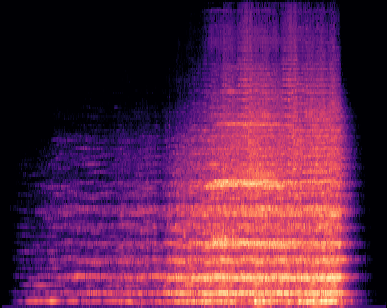
\includegraphics[width=\linewidth]{slike/horror30.png}
	Horror
\end{minipage}%
\end{frame}






\begin{frame}{Rezultati}
\centering
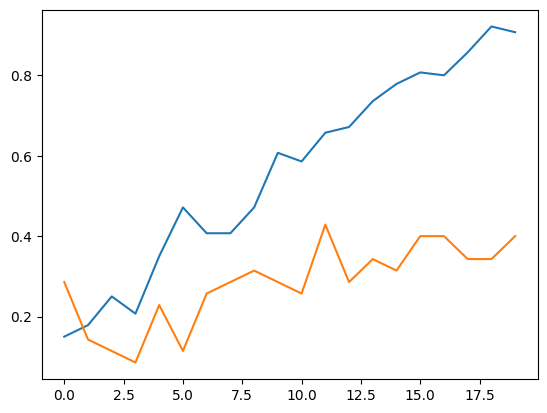
\includegraphics[width=0.4\linewidth]{slike/1acc.png}
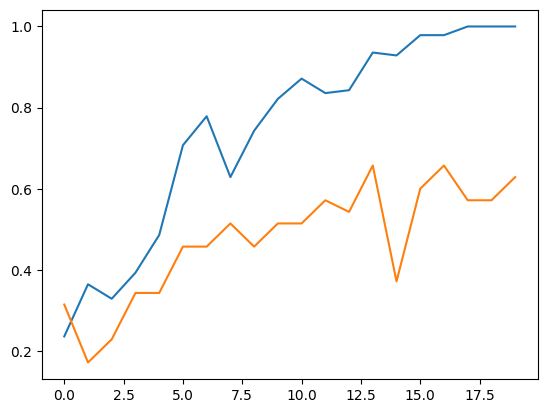
\includegraphics[width=0.4\linewidth]{slike/2acc.png}
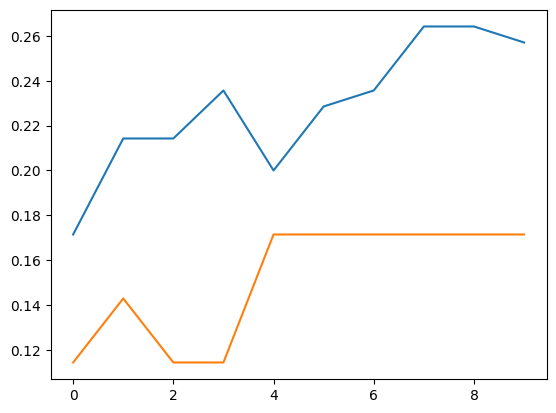
\includegraphics[width=0.4\linewidth]{slike/3acc.png}
\end{frame}

\begin{frame}{Zaključak}
Cilj projekta bio je istraživanje i razvoj modela za klasifikaciju filmskih žanrova na osnovu karakteristika muzike iz filmova. Muzika ima značajan uticaj na emotivnu percepciju i atmosferu filma, pa je razumevanje kako se ove karakteristike prepoznaju i klasifikuju mogu biti od značaja. Prikupljanje podataka za ovu vrstu zadatka je izazovno, ali od ključne važnosti. Pažljivo je kreiran dataset od 250 pesama, sa po 50 pesama za svaki od pet analiziranih žanrova. Ovaj dataset je bio osnova za obuku i testiranje modela. Za obradu spektrograma muzike, korišćena je konvolutivna neuronska mreža (CNN). Razvijena su tri različita modela sa različitim arhitekturama kako bi se istražila efikasnost u klasifikaciji žanrova.
\end{frame}

\begin{frame}{Hvala na pažnji}
\centering
\Huge Hvala na pažnji!
\end{frame}

\end{document}